\documentclass[aspectratio=169, 11pt]{beamer}

% --- Packages & Setup ---
\usepackage[utf8]{inputenc}
\usepackage[T1]{fontenc}
\usepackage[table]{xcolor}
\usepackage{booktabs}
\usepackage{graphicx}
\usepackage{tikz} % Required for the corner box
\usetikzlibrary{calc,arrows.meta,positioning,shapes.geometric}
\usepackage{array}
\usepackage{pgfplots}
\pgfplotsset{compat=1.17}

% Try loading Open Sans; fallback if missing
\IfFileExists{opensans.sty}{\usepackage[default,scale=0.95]{opensans}}{}

% --- Branding Colors ---
\definecolor{amritaMaroon}{HTML}{A4123F}

% --- Theme Setup ---
\usetheme{Madrid}
\usecolortheme[named=amritaMaroon]{structure}
\setbeamertemplate{navigation symbols}{}
\setbeamertemplate{footline}[frame number]
\setbeamertemplate{itemize items}[circle]
\setbeamerfont{footnote}{size=\tiny}

\newcommand{\srcnote}[1]{{\footnotesize\color{gray}\textit{#1}}}

\begin{document}

% --- CUSTOM TITLE SLIDE (Research) ---
\begin{frame}
    % Corner Box Indicator
    \begin{tikzpicture}[remember picture,overlay]
        \node[fill=amritaMaroon, text=white, font=\bfseries\footnotesize, anchor=north east, rounded corners=2pt, inner sep=5pt]
        at ($(current page.north east) + (-0.2cm,-0.2cm)$)
        {Type 1: Research Project};
    \end{tikzpicture}

    \centering
    \IfFileExists{logo.png}{\includegraphics[width=3.5cm]{logo.png}}{}
    \vspace{0.3cm}

    {\Large \textbf{\textcolor{amritaMaroon}{An AI-Driven, Blockchain-Anchored Cyber Deception \\ Framework for Adaptive Honeypot Defense}}} \\
    \vspace{0.2cm}
    {\normalsize \textbf{Team Number: [XX]}} \\
    \vspace{0.5cm}

    % Student Table
    \begin{table}
        \centering
        \small
        \renewcommand{\arraystretch}{1.2}
        \begin{tabular}{|c|c|l|}
            \hline
            \textbf{S.No} & \textbf{Register Number} & \textbf{Student Name} \\
            \hline
            1 & CB.EN.U4CSE23XXX & Student Name 1 \\
            \hline
            2 & CB.EN.U4CSE23XXX & Student Name 2 \\
            \hline
            3 & CB.EN.U4CSE23XXX & Student Name 3 \\
            \hline
            4 & CB.EN.U4CSE23XXX & Student Name 4 \\
            \hline
        \end{tabular}
    \end{table}
    \vspace{0.3cm}

    Guide: \textbf{[Guide Name]} \\
    {\footnotesize Designation, Department of CSE}

    \vspace{0.5cm}
    {\footnotesize \today}
\end{frame}

% ============================================================
\section{Problem Statement}
\begin{frame}{Problem Statement}
    Traditional honeypots rely on \textbf{static, deterministic response tables} --- efficient at scale, but fragile against fingerprinting.
    \begin{itemize}
        \item \textbf{Fingerprintable by design.} Prior work shows automated probing can distinguish static honeypots (Cowrie, Kippo, Dionaea) from real systems with near-perfect accuracy in a \emph{single packet exchange}.
        \vspace{2mm}
        \item \textbf{Single-protocol LLM deception.} Existing LLM-backed honeypots (shelLM, HoneyGPT) are concentrated on SSH/terminal sessions only --- no shared framework spans multiple heterogeneous protocols.
        \vspace{2mm}
        \item \textbf{Untrustworthy forensic logs.} A compromised honeypot host can have its own logs silently edited by the attacker, destroying the evidentiary value of captured telemetry.
    \end{itemize}
\end{frame}

% ============================================================
\section{Objective}
\begin{frame}{Objective}
    To build a deployable, multi-protocol deception framework that stays convincing under sustained probing and produces a tamper-evident audit trail:
    \begin{itemize}
        \item \textbf{Cover five distinct attack surfaces} --- SSH, an internal AI API, PostgreSQL, an Ethereum JSON-RPC node, and Jenkins CI/CD --- behind one shared response engine.
        \item \textbf{Stay fast where it can, smart where it must.} Answer routine traffic ($\approx$80\%) at millisecond latency via a static path; reserve LLM generation for genuinely novel input.
        \item \textbf{Make every interaction context-aware.} Replace canned responses with an LLM engine that is session-history-aware and intent-classified.
        \item \textbf{Anchor forensic integrity independently of the host.} Hash and commit every log entry to a separate blockchain so tampering is detectable even if the honeypot itself is compromised.
        \item \textbf{Evaluate honestly.} Measure latency, throughput, response diversity, and realism as separate axes across successively larger and more realistic datasets --- and report failures, not just favorable numbers.
    \end{itemize}
\end{frame}

% ============================================================
\section{Related Work}
\begin{frame}{Research Gaps We Address}
    \begin{itemize}
        \item \textbf{LLM deception is single-protocol.} shelLM, HoneyGPT, and related 2023--2025 work apply LLM response generation only to SSH/terminal sessions; no prior system applies one LLM engine uniformly across five heterogeneous protocol types.
        \vspace{2mm}
        \item \textbf{Tamper-evident logging is generic, not honeypot-specific.} Blockchain hash-anchoring is established in digital forensics (evidence tracking, cloud VM investigation), but we found no honeypot-specific paper combining hash-anchoring with decoy logging.
        \vspace{2mm}
        \item \textbf{Realism is rarely benchmarked rigorously.} Prior LLM-honeypot papers report a single self-evaluated accuracy figure (e.g. HoneyGPT's self-reported $\approx$96\%); few report latency/throughput trade-offs or scale-dependent failure modes.
    \end{itemize}
\end{frame}

\begin{frame}{Comparison Against Cited Systems}
    \scriptsize
    \renewcommand{\arraystretch}{1.3}
    \begin{tabular}{|p{1.7cm}|p{2.0cm}|p{3.3cm}|p{2.3cm}|p{1.7cm}|}
        \hline
        \textbf{System} & \textbf{Interaction} & \textbf{AI/LLM Responses} & \textbf{Protocols} & \textbf{Tamper-evident} \\
        \hline
        Cowrie & Medium/High & No (experimental single-tier LLM fallback exists) & SSH, Telnet & No \\
        \hline
        T-Pot & Mixed (orchestrator) & No -- aggregation only & Broad (bundled daemons) & No \\
        \hline
        Dionaea & Low--Medium & No & SMB, MySQL, SIP, FTP, TFTP & No \\
        \hline
        shelLM & High (SSH only) & Yes -- full LLM shell session & SSH only & Not addressed \\
        \hline
        HoneyGPT & High (terminal) & Yes -- GPT-3.5/4 via Cowrie proxy & SSH/terminal only & Not addressed \\
        \hline
        \textbf{This work} & \textbf{High, all 5} & \textbf{Yes -- 3-tier, session-aware, uniform across 5 protocols} & \textbf{SSH, AI API, SQL, Web3 RPC, CI/CD} & \textbf{Yes -- SHA-256 + Ethereum anchor} \\
        \hline
    \end{tabular}
    \vspace{2mm}
    \srcnote{Table I, paper Section II.F}
\end{frame}

% ============================================================
\section{Architecture}
\begin{frame}{System Architecture --- Overview}
    Six components; only the proxy and dashboard face the network. All else communicates over an isolated internal Docker network.
    \begin{center}
    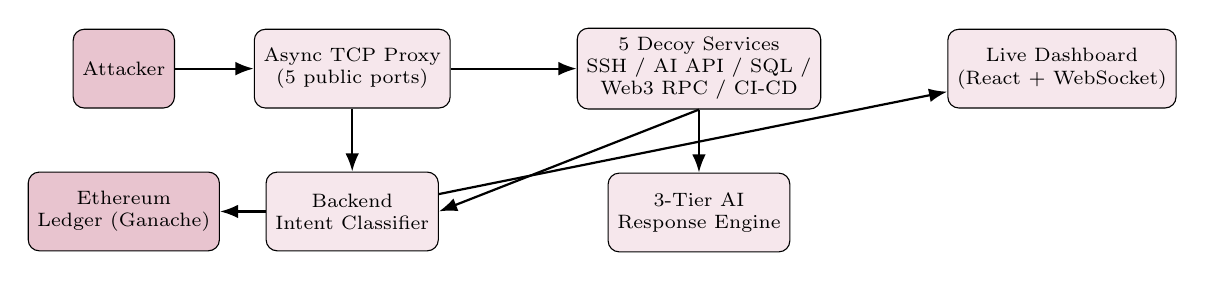
\begin{tikzpicture}[
        node distance=8mm and 10mm,
        box/.style={draw, rounded corners, fill=amritaMaroon!10, align=center, minimum height=1cm, font=\scriptsize},
        arr/.style={-{Latex}, thick}
    ]
        \node[box, fill=amritaMaroon!25] (attacker) {Attacker};
        \node[box, right=of attacker] (proxy) {Async TCP Proxy\\(5 public ports)};
        \node[box, right=1.6cm of proxy, minimum width=2.6cm] (decoys) {5 Decoy Services\\SSH / AI API / SQL /\\Web3 RPC / CI-CD};
        \node[box, below=of decoys] (engine) {3-Tier AI\\Response Engine};
        \node[box, below=of proxy] (backend) {Backend\\Intent Classifier};
        \node[box, below=of attacker, fill=amritaMaroon!25] (chain) {Ethereum\\Ledger (Ganache)};
        \node[box, right=1.6cm of decoys, minimum width=2.2cm] (dash) {Live Dashboard\\(React + WebSocket)};

        \draw[arr] (attacker) -- (proxy);
        \draw[arr] (proxy) -- (decoys);
        \draw[arr] (decoys) -- (engine);
        \draw[arr] (proxy) -- (backend);
        \draw[arr] (decoys.south) -- (backend.east);
        \draw[arr] (backend) -- (chain);
        \draw[arr] (backend) -- (dash);
    \end{tikzpicture}
    \end{center}
    \srcnote{Paper Section III}
\end{frame}

\begin{frame}{Five Decoy Services}
    \scriptsize
    \renewcommand{\arraystretch}{1.05}
    \setlength{\tabcolsep}{4pt}
    \begin{tabular}{|l|l|p{7.4cm}|}
        \hline
        \textbf{Decoy} & \textbf{Port / Protocol} & \textbf{Role} \\
        \hline
        \texttt{shadow-shell} & 2222 / SSH & Real \texttt{asyncssh} server; accepts any credentials; shell prompt for \texttt{dbadmin@corp-prod-db-01}; commands route through AI engine \\
        \hline
        \texttt{oracle-ai} & 8080 / REST & FastAPI chat/predict endpoints for a fictitious internal model; prompt-injection bait \\
        \hline
        \texttt{vault-sql} & 5433 / Postgres & Real seeded Postgres instance with synthetic records + honeytoken API keys (OpenAI/GitHub/AWS-formatted) \\
        \hline
        \texttt{ledger-trap} & 8545 / JSON-RPC & Ethereum node decoy; static replies for common RPC calls, AI engine for uncommon ones \\
        \hline
        \texttt{forge-ci} & 9090 / HTTP & Jenkins-style CI/CD endpoints faking a working pipeline; supply-chain bait \\
        \hline
    \end{tabular}
    \vspace{1mm}
    \srcnote{Paper Section III.B}
\end{frame}

\begin{frame}{Three-Tier AI Response Engine}
    Expensive LLM calls are reserved for genuinely novel input.
    \begin{center}
    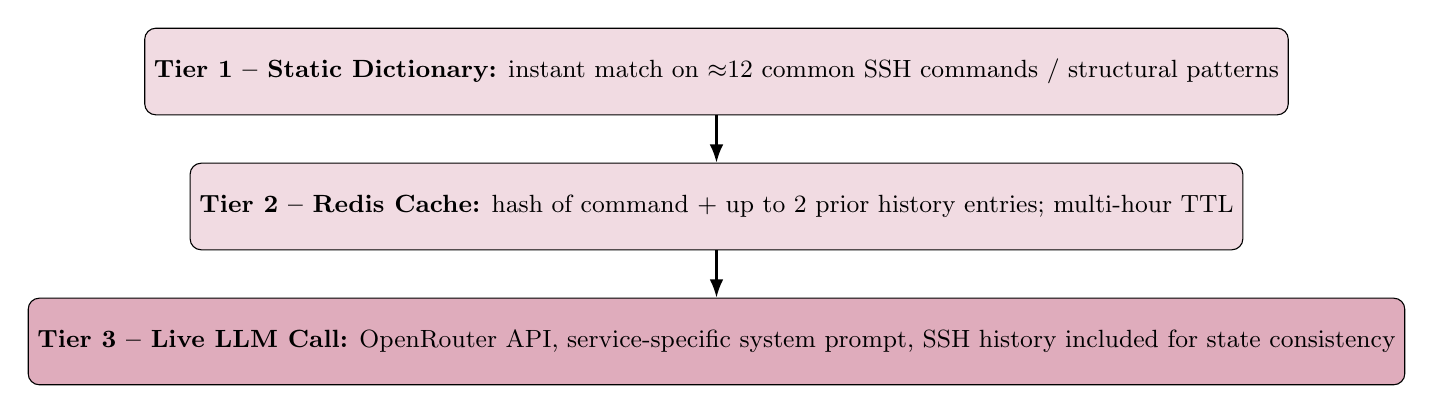
\begin{tikzpicture}[
        node distance=6mm,
        tier/.style={draw, rounded corners, fill=amritaMaroon!15, minimum width=10.5cm, minimum height=1.1cm, align=left, font=\small},
        arr/.style={-{Latex}, thick}
    ]
        \node[tier] (t1) {\textbf{Tier 1 -- Static Dictionary:} instant match on $\approx$12 common SSH commands / structural patterns};
        \node[tier, below=of t1] (t2) {\textbf{Tier 2 -- Redis Cache:} hash of command + up to 2 prior history entries; multi-hour TTL};
        \node[tier, below=of t2, fill=amritaMaroon!35] (t3) {\textbf{Tier 3 -- Live LLM Call:} OpenRouter API, service-specific system prompt, SSH history included for state consistency};
        \draw[arr] (t1) -- (t2);
        \draw[arr] (t2) -- (t3);
    \end{tikzpicture}
    \end{center}
    \vspace{2mm}
    \textbf{Intent classification:} keyword-based, 8 categories (SQLi, privesc, reverse shell, cryptomining, prompt injection, supply-chain, recon, unknown) --- a rule-based baseline, reported as a known limitation.
    \srcnote{Paper Section III.C--D}
\end{frame}

\begin{frame}{Blockchain-Anchored Logging}
    \begin{itemize}
        \item Every log entry (\texttt{POST /api/log}) is timestamped, intent-classified, serialized with sorted keys, and \textbf{SHA-256 hashed}.
        \item The hash is anchored via a \textbf{zero-value self-transaction} on a local Ethereum chain (Ganache).
        \item Stored in a bounded Redis list; broadcast over WebSocket to the live dashboard.
        \item Because the hash lives on an independently operated ledger, any later edit to the stored log is detectable by re-hashing and comparing --- \textbf{without trusting the honeypot host's own integrity}.
    \end{itemize}
    \vspace{3mm}
    \begin{block}{\small Integrity Test Result}
        \small A log entry (hash \texttt{356b7496...33a9a1}) was anchored, fetched back, and re-hashed --- identical. A tampered copy (\texttt{"sudo cat /etc/shadow"} $\to$ \texttt{"ls -la"}) produced a different hash (\texttt{7530fb00...0d9d394}), confirming tamper-evidence.
    \end{block}
    \srcnote{Paper Section III.E, V.D}
\end{frame}

% ============================================================
\section{Evaluation Methodology}
\begin{frame}{Evaluation Methodology}
    Evaluated against the system's own static fast-path (functionally equivalent to Cowrie) vs. its LLM-backed dynamic path.
    \begin{itemize}
        \item \textbf{Four metrics, kept separate:}
        \begin{itemize}
            \item Latency / throughput (30 static trials, 20 dynamic trials)
            \item Response diversity --- fraction of distinct outputs per service
            \item LLM-judge realism score --- independent 70B judge (distinct from 8B generator), 1--5 rubric, 30-payload sample
            \item Blockchain integrity --- direct tamper test
        \end{itemize}
        \item \textbf{Four successive runs}, each scaling up dataset realism:
        \begin{enumerate}
            \item 100 hand-written payloads (baseline)
            \item Same dataset, after an optimization pass
            \item 200 real, publicly-documented payloads
            \item 1{,}328 real payloads (scaled corpora)
        \end{enumerate}
        \item Explicitly \textbf{not} a single composite accuracy figure --- trade-offs and failures are reported, not hidden.
    \end{itemize}
    \srcnote{Paper Section IV}
\end{frame}

% ============================================================
\section{Results}
\begin{frame}{Run 1: Initial Baseline (100 Hand-Written Payloads)}
    \scriptsize
    \renewcommand{\arraystretch}{1.2}
    \begin{tabular}{|l|c|c|}
        \hline
        \textbf{Metric} & \textbf{Static} & \textbf{Dynamic} \\
        \hline
        Mean latency & 0.4 ms & 4{,}028 ms (4.03 s) \\
        \hline
        Median latency & 0.4 ms & 3{,}529 ms (3.53 s) \\
        \hline
        Throughput (req/s) & 2{,}500 & 0.25 \\
        \hline
        Diversity ratio (mean) & $\approx$0 & 0.99 (0.95--1.00) \\
        \hline
    \end{tabular}
    \vspace{3mm}
    \normalsize
    LLM-judge realism: \textbf{4.38/5} ($\sigma=1.28$, $n=24$ of 30 parsed)
    \vspace{2mm}
    \srcnote{Table II, paper Section V.A}
\end{frame}

\begin{frame}{Run 2: Optimization Pass}
    \textbf{Two fixes identified by profiling:}
    \begin{itemize}
        \item HTTP connection pooling (was opening a fresh TCP+TLS handshake to OpenRouter \emph{every request})
        \item Generation-length cap tuned from 150 $\to$ 60 tokens (150 tok $\approx$5.3s, 80 tok $\approx$3.4s, 40 tok $\approx$2.0s --- generation length dominates latency)
        \item Static SSH dictionary widened with 12 more recon commands
    \end{itemize}
    \vspace{3mm}
    \scriptsize
    \renewcommand{\arraystretch}{1.2}
    \begin{tabular}{|l|c|c|c|}
        \hline
        \textbf{Metric} & \textbf{Before} & \textbf{After} & \textbf{Change} \\
        \hline
        Dynamic mean latency & 4.03 s & 1.35 s & $\approx3\times$ \\
        \hline
        Dynamic throughput (seq.) & 0.25 rps & 0.74 rps & $\approx3\times$ \\
        \hline
        Static throughput & 2{,}500 rps & 3{,}333 rps & $+33\%$ \\
        \hline
        LLM-judge realism & 4.38/5 (24/30) & 4.00/5 (30/30) & $-0.38$ \\
        \hline
    \end{tabular}
    \srcnote{Table III, paper Section V.B}
\end{frame}

\begin{frame}{Latency Comparison --- Before vs. After}
    \begin{center}
    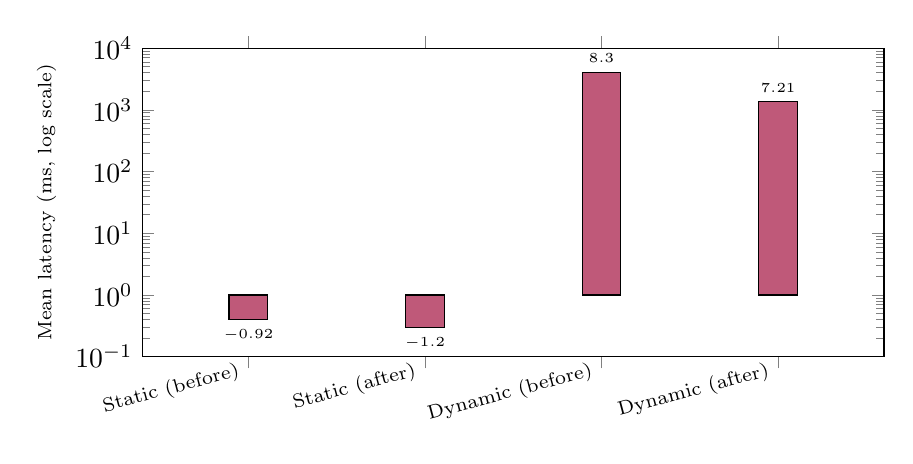
\begin{tikzpicture}
        \begin{axis}[
            ybar, bar width=14pt, width=11cm, height=5.5cm,
            ymode=log, ymin=0.1, ymax=10000,
            symbolic x coords={Static (before),Static (after),Dynamic (before),Dynamic (after)},
            xtick=data, x tick label style={font=\scriptsize, rotate=15, anchor=east},
            ylabel={Mean latency (ms, log scale)}, ylabel style={font=\scriptsize},
            nodes near coords, nodes near coords style={font=\tiny},
            enlarge x limits=0.2,
            ]
            \addplot[fill=amritaMaroon!70] coordinates {(Static (before),0.4) (Static (after),0.3) (Dynamic (before),4028) (Dynamic (after),1351)};
        \end{axis}
    \end{tikzpicture}
    \end{center}
    \srcnote{Fig. 1, paper Section V.B}
\end{frame}

\begin{frame}{Decoy-Layer Connection Pooling (All 5 Decoys)}
    \scriptsize
    \renewcommand{\arraystretch}{1.2}
    \begin{tabular}{|l|c|c|c|}
        \hline
        \textbf{Decoy} & \textbf{Before (mean)} & \textbf{After (mean)} & \textbf{$\Delta$} \\
        \hline
        oracle-ai & 6.15 ms & 4.28 ms & $-30.4\%$ \\
        \hline
        vault-sql & 0.69 ms & 0.41 ms & $-41.4\%$ \\
        \hline
        ledger-trap & 5.96 ms & 4.20 ms & $-29.5\%$ \\
        \hline
        forge-ci & 6.95 ms & 6.71 ms & $-3.4\%$ \\
        \hline
        shadow-shell & 7.91 ms & 4.64 ms & $-41.3\%$ \\
        \hline
    \end{tabular}
    \vspace{3mm}
    \normalsize
    Real and consistent improvement on 4 of 5 decoys; \texttt{forge-ci} barely moves since it always routes through the AI engine regardless of decoy-layer pooling.
    \srcnote{Table IV, paper Section V.C}
\end{frame}

\begin{frame}{Runs 3--4: Real-World Payload Datasets}
    The hand-written dataset was replaced with \textbf{real, publicly-documented} attack payloads (payload-box, PayloadsAllTheThings, SecLists), scaled 100 $\to$ 200 $\to$ 1{,}328 payloads.
    \vspace{2mm}
    \scriptsize
    \renewcommand{\arraystretch}{1.2}
    \begin{tabular}{|l|c|c|}
        \hline
        \textbf{Metric} & \textbf{200-item} & \textbf{1{,}328-item} \\
        \hline
        Dynamic latency (mean) & 2.06 s & 1.95 s \\
        \hline
        Concurrent throughput (10 sessions) & 1.62 req/s & 3.05 req/s \\
        \hline
        Response diversity -- ssh & 0.925 & 0.964 \\
        \hline
        Response diversity -- sql & 1.00 & 0.978 \\
        \hline
        Response diversity -- web3 & 0.80 & 0.833 \\
        \hline
        Response diversity -- cicd & 0.90 & 1.00 \\
        \hline
        \rowcolor{amritaMaroon!15} Response diversity -- \textbf{api} & \textbf{0.70} & \textbf{0.46} \\
        \hline
        LLM-judge realism (mean) & 4.03/5 & 3.37/5 \\
        \hline
    \end{tabular}
    \srcnote{Table VI, paper Section V.E--F}
\end{frame}

\begin{frame}{Response Diversity by Decoy Service}
    \begin{center}
    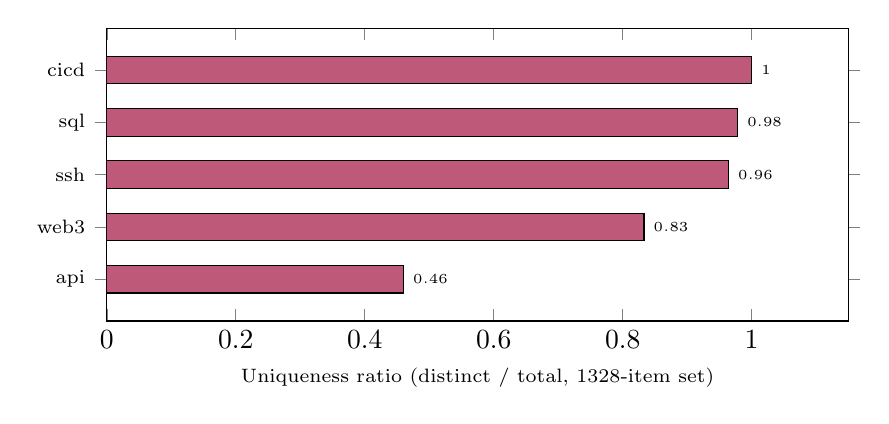
\begin{tikzpicture}
        \begin{axis}[
            xbar, bar width=10pt, width=11cm, height=5.3cm,
            xmin=0, xmax=1.15,
            symbolic y coords={api,web3,ssh,sql,cicd},
            ytick=data, y tick label style={font=\scriptsize},
            xlabel={Uniqueness ratio (distinct / total, 1328-item set)}, xlabel style={font=\scriptsize},
            nodes near coords, nodes near coords style={font=\tiny},
            enlarge y limits=0.2,
            ]
            \addplot[fill=amritaMaroon!70] coordinates {(0.46,api) (0.833,web3) (0.964,ssh) (0.978,sql) (1.00,cicd)};
        \end{axis}
    \end{tikzpicture}
    \end{center}
    \textbf{api} is the clear outlier --- the model frequently collapses to a generic \textit{"invalid request"} reply on real XXE / Log4Shell strings instead of emulating a plausible vulnerable-parser response.
    \srcnote{Fig. 5, paper Section V.C, V.F}
\end{frame}

\begin{frame}{The Benchmark-Harness Bug}
    A genuine measurement bug was found and fixed during the real-dataset re-run.
    \begin{itemize}
        \item The concurrent-throughput benchmark reused payloads \textbf{already sent once earlier} in the same run.
        \item Because the Redis cache key derives from command + history, these were guaranteed cache \textbf{hits} --- so the ``800 req/s'' figure measured Redis latency, not LLM latency.
        \item \textbf{Fix:} append a fresh UUID nonce to every payload immediately before firing the concurrent batch.
    \end{itemize}
    \vspace{2mm}
    \scriptsize
    \renewcommand{\arraystretch}{1.2}
    \begin{tabular}{|l|c|c|}
        \hline
        \textbf{Metric} & \textbf{First-reported (bug)} & \textbf{Corrected} \\
        \hline
        Concurrent throughput (10 sessions) & 800.3 req/s & 3.05 req/s \\
        \hline
        Mean per-request latency & 8.2 ms & 2.62 s \\
        \hline
    \end{tabular}
    \vspace{2mm}

    \footnotesize Reported explicitly rather than silently substituted --- a 3-order-of-magnitude bug is itself a methodological finding.
    \vspace{1mm}
    \srcnote{Table V, paper Section V.E}
\end{frame}

\begin{frame}{Realism Score Distribution (Post-Optimization, n=30)}
    \begin{center}
    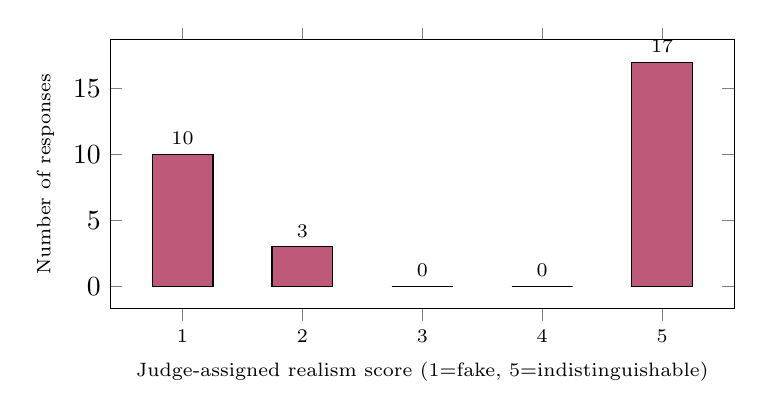
\begin{tikzpicture}
        \begin{axis}[
            ybar, bar width=22pt, width=9.5cm, height=5cm,
            symbolic x coords={1,2,3,4,5},
            xtick=data, xlabel={Judge-assigned realism score (1=fake, 5=indistinguishable)},
            xlabel style={font=\scriptsize}, x tick label style={font=\scriptsize},
            ylabel={Number of responses}, ylabel style={font=\scriptsize},
            nodes near coords, nodes near coords style={font=\scriptsize},
            enlarge x limits=0.15,
            ]
            \addplot[fill=amritaMaroon!70] coordinates {(1,10) (2,3) (3,0) (4,0) (5,17)};
        \end{axis}
    \end{tikzpicture}
    \end{center}
    \srcnote{Fig. 3, paper Section V.B}
\end{frame}

\begin{frame}{Key Finding: The API Decoy's Realism Failure}
    At the 1{,}328-item scale, \textbf{9 of 11} sampled \texttt{api} responses scored 1--2/5 --- versus near-uniform 5/5 for ssh, sql, and web3 in the same sample.
    \begin{block}{\small Most Consequential Result}
        \small One sampled response was found to contain an \textbf{explicit AI safety disclaimer} (\textit{``Contains an explicit disclaimer about not generating harmful responses''}) --- a hard deception failure, not a minor realism deduction. It signals \textit{``this is not a real system''} to exactly the attentive attacker the framework is designed to hold.
    \end{block}
    \vspace{2mm}
    \begin{itemize}
        \item This failure was \textbf{invisible} in the original 100-payload and even the 200-payload runs --- it only became unambiguous at the largest (1{,}328-item) scale.
        \item Root cause: the hosted model's own safety training bleeds through the deception persona on XML/JNDI-shaped adversarial input.
        \item \textbf{Actionable fix (not yet applied):} XXE/Log4Shell/SSRF-aware few-shot examples + explicit anti-disclaimer instruction in \texttt{oracle-ai}'s system prompt.
    \end{itemize}
    \srcnote{Paper Section V.F, VI}
\end{frame}

% ============================================================
\section{Discussion}
\begin{frame}{Discussion}
    \begin{itemize}
        \item \textbf{Not a drop-in replacement} for high-volume, low-interaction scanning honeypots --- static-path systems remain appropriate there.
        \item \textbf{Targeted use case:} high-interaction deception against a human operator or a sophisticated, low-volume tool, where multi-second latency is plausibly attributable to network/server load.
        \item \textbf{Concurrency is real but modest:} 10 concurrent sessions complete in 3.28 s wall-clock (not $\approx$19.5 s), but this is far short of the originally (buggy) reported capacity.
        \item \textbf{The AI-persona failure is structural, not incidental:} any decoy built on a hosted, safety-tuned model inherits an alignment layer that is directly adversarial to the deception goal on concerning inputs.
        \item Blockchain anchoring assumes the ledger is outside attacker reach --- reasonable for an internal Ganache deployment, not evaluated against an adversary who also compromises the chain client.
    \end{itemize}
    \srcnote{Paper Section VI}
\end{frame}

% ============================================================
\section{Limitations \& Future Work}
\begin{frame}{Limitations \& Future Work}
    \begin{itemize}
        \item LLM-judge realism score is an \textbf{automated proxy} --- needs human-subject validation (protocol specified in paper Appendix A, not yet executed).
        \item Real-payload datasets (up to 1{,}328 items) are still \textbf{not live-traffic captures} --- no multi-step sessions, timing, or evasion behavior.
        \item \texttt{web3} and \texttt{cicd} datasets remain small (18, 10 payloads) --- no comparably large real corpus exists for those surfaces; a genuine coverage gap.
        \item Intent classification is \textbf{keyword-based} --- will misclassify obfuscated/novel patterns; a learned classifier is a natural extension.
        \item No longitudinal live-internet deployment yet; concurrent-throughput tested only at a single burst level (10 sessions).
        \item \textbf{Immediate next step:} rewrite \texttt{oracle-ai}'s system prompt with XXE/JNDI-aware few-shot examples and an explicit anti-disclaimer instruction, then re-measure.
    \end{itemize}
    \srcnote{Paper Section VII}
\end{frame}

% ============================================================
\section{References}
\begin{frame}[allowframebreaks]{References}
    \scriptsize
    \begin{thebibliography}{99}
        \bibitem{vetterl} A. Vetterl and R. Clayton, ``Bitter Harvest: Systematically Fingerprinting Low- and Medium-interaction Honeypots at Internet Scale,'' \textit{Proc. 12th USENIX WOOT}, 2018.
        \bibitem{multistage} ``Gotta Catch 'em All: A Multistage Framework for Honeypot Fingerprinting,'' \textit{ACM Digital Threats: Research and Practice}, 2023, arXiv:2109.10652.
        \bibitem{shellm} M. Sladi\'{c}, V. Valeros, C. Catania, and S. Garcia, ``LLM in the Shell: Generative Honeypots,'' \textit{Proc. IEEE EuroS\&PW}, 2024, arXiv:2309.00155.
        \bibitem{honeygpt} Z. Wang et al., ``HoneyGPT: Breaking the Trilemma in Terminal Honeypots with Large Language Model,'' arXiv:2406.01882, 2024.
        \bibitem{mckee} F. McKee and D. Noever, ``Chatbots in a Honeypot World,'' arXiv:2301.03771, 2023.
        \bibitem{llmhoneypot} ``LLM Honeypot: Leveraging Large Language Models as Advanced Interactive Honeypot Systems,'' arXiv:2409.08234, 2024.
        \bibitem{blockchainforensic} ``Blockchain-Based Evidence Tracking System for Forensic Integrity and Secure Chain of Custody,'' IEEE, 2025.
        \bibitem{cloudvm} ``Blockchain-based tamper-proof and transparent investigation model for cloud VMs,'' \textit{The Journal of Supercomputing}, Springer, 2022.
        \bibitem{peerj} ``A novel intelligent cyber threat detection system with blockchain-enforced immutable forensic auditability,'' \textit{PeerJ Computer Science}, 2025.
        \bibitem{mitre} MITRE, ``MITRE Engage: A Framework and Community for Cyber Deception,'' 2022.
        \bibitem{cowrie} Cowrie SSH/Telnet Honeypot, GitHub repository.
        \bibitem{sok} ``SoK: Honeypots and Large Language Models --- Systematization of a Growing Intersection,'' arXiv:2510.25939, 2025.
    \end{thebibliography}
\end{frame}

% --- THANK YOU ---
\begin{frame}
    \centering
    {\Huge \textbf{\textcolor{amritaMaroon}{Thank You}}}
\end{frame}

\end{document}